\documentclass{article}
\usepackage[margin=1in]{geometry}
\usepackage{comment}
\usepackage{amssymb,amsmath}
\usepackage{floatrow}
\usepackage{graphicx}
\usepackage{caption}
\usepackage{subcaption}
\usepackage{listings}
\usepackage{algpseudocode}
\usepackage{algorithm}
\usepackage{program}
\usepackage{color}
\usepackage{enumitem}
\usepackage{cite}
%\setlist{nolistsep}

\algblockdefx[ForEach]{ForEach}{EndFor} %
	[1]{\textbf{for each} $#1$ \textbf{do}} %
	[0]{\textbf{end for}}

\algblockdefx[ForEachIn]{ForEachIn}{EndFor} %
	[2]{\textbf{for each} $#1$ \textbf{in} $#2$ \textbf{do}} %
	[0]{\textbf{end for}}

\floatsetup{
  heightadjust=object,
  valign=t
}

\algloopdefx{SingleIf}[1]{\textbf{if} \textsl{#1} \textbf{then}}
\algnewcommand\algorithmicin{\textbf{in}}

\title{EECS281A Fall 2012 Final Project: \\ Machine Learning in Auto-tuning Stencil Computation on GPU}

\author{Penporn Koanantakool}

\begin{document}
\maketitle

\section{Introduction} % what is the problem. what is our solution.

Tuning applications could be considered an art form. It requires expertise in identifying important underlying factors and understanding their correlation. Auto-tuning is an attempt to find such well-performing configurations automatically. Since the search space is often too large to test exhausibly, machine learning is well-adopted in this field to reduce time to solution, mostly by predicting or modeling program performance for each configuration instead of actually running it.

As of current, althought there are many researches on using machine learning in auto-tuning, not many of them cover architectures other than CPUs (Central Processing Units). In addition, even with the existing frameworks for CPU ones are considerably diverge and are more of studying a certain algorithm on a certain application. This leaves an open question of what algorithm to chose for each application. In this project, I compare how well selected machine learning algorithms assist tuning a stencil computation application on GPU. Selected algorithms are Gradient Boosted Regression Tree, Kernel Ridge Regression (KRR), Support Vector Machine (SVM), and Kernel Canonical Correlation Analysis (KCCA).

% How well they perform against each other


\section{Background}
In this section, we start with formal definitions of auto-tuning and stencil computation, followed by a brief introduction to GPU architecture and its programming model. Then we end the section with details on selected algorithms, which are known to work with auto-tuning.

\subsection{Auto-tuning}
Given a program with n tunable parameters, we call a tuple of values $(x_1, ..., x_n)$ corresponding to each parameter a \emph{configuration}. The set of all possible configurations is called a \emph{parameter space} or \emph{search space}. Auto-tuning  is the problem of finding the configuration that gives the best performance. Although the performance metric can be any values of interest, most tunings' metric is the running time (lowest is best), and so do this project.

There are various approaches to auto-tuning. Of course the most na\"{i}ve one would be to actually run the application for all possible configurations and pick the best results. Unfortunately, the search space is often too large for this approach to be feasible. These approaches could be classified into 3 broad categories \cite{inpar2012}:
\begin{description}
	\item[Model-based optimization] involves analytically constructing a performance model specific to the underlying hardware and does code transformation accordingly. However, such models are generally difficult to build.
	\item[Empirical optimization] searches for the best configuration by picking one initial configuration, generating code, benchmarking them on the actual hardware, determining the next configuration to be tested and repeat the whole process until an end condition is satisfied. It takes considerably more time than the model-based optimization and its performance depends heavily on the search method. There is a tradeoff between faster running time and more accuracy.
	\item[Predictive optimization] combines the first to approaches, enhancing the empirical optimization modeling/predicting the running time instead of actually running time. In this project we will use this approach and use machine learning algorithms for the prediction part.
\end{description}

\subsection{Stencil Computation}
Stencil computation is used in wide range applications from solving system of Partial Differential Equations (PDEs) to filtering in image processing. It iterates over timesteps and performs stencil operations on all points in a grid in each iteration. Stencil operation on a point updates its value to a linear combination\footnote{In other words, weighted sum} of its nearest neighbors, within a fixed distance, and sometimes itself. An example 3D 25-point stencil is shown in Figure~\ref{fig:25-point_stencil}. We will use this stencil in our benchmark application.

\begin{figure*}[!t]
\centering
\includegraphics[width=0.25\textwidth]{./images/25-point-stencil.pdf}
\caption{Illustration of a 3D 25-point stencil (4 neighbors in each direction). (Courtesy of NVIDIA)}
\label{fig:25-point_stencil}
\end{figure*}

Stencil computation is mostly bandwidth-bound, since they rely on many points around while the computation is trivial.

\subsection{NVIDIA GPU and CUDA Programming Model}
GPU (Graphical Processing Unit) is a massively parallel processor that was originally designed for just display purpose. With the introduction of programming frameworks that allows programmers to program general-purpose application on GPUs more conveniently, graphic cards quickly became one of the most popular hardware accelerators nowadays. Among all vendors, NVIDIA GPUs are the most popular and widely available.

Figure \ref{fig:gpu-arch} shows the architecture of an NVIDIA GPU. An NVIDIA GPU consists of many SIMD (Single Instruction Multiple Data) cores, dubbed Streaming Multiprocessors, and its own high-bandwidth DRAM memory. Each core has a large register file and a user-managed cache called \textbf{shared memory}. There are three types of out-of-core memory: global memory, constant memory, and texture memory. Global memory is the largest one and is used in general purpose. The latter two are read-only.

\begin{figure*}[!t]
\centering
\includegraphics[width=0.25\textwidth]{./images/gpu-architecture.pdf}
\caption{NVIDIA GPU architecture (Courtesy of NVIDIA)}
\label{fig:gpu-arch}
\end{figure*}

The programming model for NVIDIA GPUs is called CUDA (Compute Unified Device Architecture). To program on a GPU, one needs to write a normal CPU \emph{`host'} code that calls a separate CUDA \emph{`kernel'}\footnote{Not to be confused with kernels in Statistics} code, which is simply a function to be executed simultaneously on GPU cores.

A set of all threads that is used to execute a kernel is referred to as a ``grid" in CUDA context. For each grid, the threads are divided into groups called thread blocks (for scalability reasons ..cite CUDA Programmming Handbook). Threads in the same block will be executed on the same GPU core, and will be able to share resources and synchronize. The block size affects the resources usage on a core and determines how many threads will be able to execute on the whole GPU device in total, and thus it is one of the most important tuning parameters of a GPU program.

Given that a stencil computation is bandwidth bound, the keys to optimize it are simply
\begin{enumerate}
	\item Optimizing for highest memory bandwidth by
		\begin{enumerate}
			\item Coalescing memory reads from global memory.
			\item Design load and store pattern to minimize extra reads from global memory. For example, use shared memory to share data among threads in the same block, and order the usage pattern so that we don't need to load the same data again later in the computation.
		\end{enumerate}
	\item Utilizing as many computing resources as possible
\end{enumerate}

\subsection{Machine Learning in Auto-tuning Stencil Computation}
There are several auto-tuning researches on stencil computation on GPUs, but they don't utilize Machine Learning. Datta et al.\ and Kamil et al.\ explained a thorough framework to auto-tune stencil computation on various multicore architectures including NVIDIA GPUs. They used empirical optimization with iterative greedy search algorithm with heuristics. \cite{datta08, datta09, shoaib10} Zhang and Mueller recently explored auto-tuning of 3D stencil computatoin exclusively on GPUs, including GPU clusters. They exhaustively tested all configurations. \cite{zhang12}

In fact, there are few auto-tuning project on GPU that even uses machine learning. To be appear in the inaugural Innovative Parallel Computing (InPar) 2012 is a work on predictive auto-tuning on GPU by Bergstra et al.\ \cite{inpar2012} They used Boosted Regression Tree (BST) to predict program's performance and used hill-climbing (HC) search algorithm to find the best configuration. Their benchmark application was a simple spatial image filter called Filterbank correlation. They found that the predicted running times correlate very well with the results from their actual runs across 5 models of NVIDIA GPUs. They also asserted that the auto-tuning should be input-dependent, that is choosing kernels according to each input configuration.

Ganapathi et al.\ took an interesting approach in tuning stencil computation on multicore architectures, although GPU was not included. \cite{KCCA} Having set the desired performance metrics to be both energy and speed, she opted for a rather compute-intensive machine learning algorithm called Kernel Canonical Correlation Analysis (KCCA). The key idea is to project the set of configurations and the set of measured corresponding metrics onto a space that they correlate the most, and then project the best configuration of the test set onto that space, find nearest neighbors in the projected space, and then generate new (much smaller) set of configuration to be searched empirically for the best parameter. The performance the auto-tuning was able to achieve is within 1\% of and up to 18\% better than a human expert.

Observing that the BRT and KCCA algorithms perform well, I chose to study 2 regression tree algorithms and 2 kernel algorithms: (Gradient) Boosted Regression Tree, Random Forest, Kernel Ridge Regression, and Kernel Canonical Correlation Analysis.
\begin{description}
\item[Regression Trees] Regression Trees predict by recursively dividing input space to constant region. They are interesting to auto-tuning because they are non-parametric. That is, they don't need to know the probability distribution of the latent variable. Apart from quick decision time, the splitting condition can help in learning what parameters is crucial in tuning, which is always good to know regardless of how obvious they are. However, they do have drawbacks. Regression trees have high variance since each different decision at the splitting node can lead to totally different conditions later on down the tree. However, this can be avoided by additive algorithms. \emph{Boosted Regression Tree} is a committee-based algorithm that tries to create a strong learner from multiple weak learners. It iteratively combines regression trees from learning samples that are weighted so that the ones that were previously classified wrong has more weight (Learning from mistakes). \emph{Random Forest} is another way by combining random trees together.
\item[Kernel Canonical Correlation Analysis] is a kernelized version of Canonical Correlation Analysis.\cite{KICA} It is similar to PCA in essence. The algorithm is previously mentioned in last paragraph. The projection can be viewed as discovering the generating factors that lies behind two sets of data. For example, in auto-tuning configurations and observed running times are the two sets of data and the maximal correlation projection can be considered the projection of all deciding hardware and application constraints summarized in just one dimension. I'm very interested and intrigued by this. Thus, I include it here even though it seems to be an overkill for this problem. (Solving KCCA equals to solving generalized eigenvector problem, thus it has $O(n^3)$ complexity.)
\item[Kernel Ridge Regression] I add this
\end{description}



% Add KCCA if I can use it..
% Add amik paper if end up using analytic model


\section{Benchmarks}
I use two stencil kernels: a very simple one to test the water, and hypterm, a kernel from real Compressible Navier Stokes application.

\subsection{Simple Stencil}
Algorithm \ref{alg:simple} shows what the simple stencil computes. GPU algorithm will look slightly different since it will be instructions for each thread to work on just their assigned portion. Also, since stencil computation is bandwidth-bound, we have to be careful about reading data or the memory access time will dominate in most cases and that wouldn't be interesting to tune.
To make the most reuse of data, I followed NVIDIA's Micikevicius optimized approach \cite{nvidia_25p-stencil}. In essence, we create 2D thread blocks. Each thread $(i,j)$ will work on the points $x(f(i),g(j),:)$ (moving along the z direction). At the beginning, before computation, all threads in the same block coordinate on loading the plane $z=k_0$ into shared memory, then compute the stencil operation, sharing the data as illustrated in Figure \ref{fig:25-point_stencil}. Then the threads moves on to next $z=k_0+1$ altogether and coordinating on loading plan $z=k_0+1$ and so on. This way all threads can share most of the data in the xy plane and only have to pay for the data they loads in the z direction. However, this is not expensive either, since 7 of the 8 values it read in the first step is reused in the next step, and thus it only needs to load one more new value for the z direction. The full algorithm is listed in Algorithm \ref{alg:simple-gpu}. Both this and the hypterm kernel use double-precision floating-point.

\begin{algorithm}
\floatname{algorithm}{Algorithm}
\caption{\textsc{Simple Stencil on CPU}}
\label{alg:simple}
\begin{algorithmic}[1]
\State \emph{Input/Output:} $x$
\State \emph{Define $\phi_x(x,i,j,k)$:} Linear combination of $x[i-4:i+4,j,k]$
\State \emph{Define $\phi_y(x,i,j,k)$:} Linear combination of $x[i,j-4:j+4,k]$
\State \emph{Define $\phi_z(x,i,j,k)$:} Linear combination of $x[i,j,k-4:k+4]$
\For{each \emph{coordinate (i,j,k)} in $grid$}
	\State $x[i,j,k] \leftarrow -\phi_x(x,i,j,k) - \phi_y(x,i,j,k) - \phi_z(x,i,j,k)$
\EndFor
\end{algorithmic}
\end{algorithm}
\begin{algorithm}
\floatname{algorithm}{Algorithm}
\caption{\textsc{Simple Stencil on GPU (For Each Thread)}}
\label{alg:simple-gpu}
\begin{algorithmic}[1]
\State \emph{Input/Output:} $x$
\State \emph{Define $\phi_x(x,i,j,k)$, $\phi_y(x,i,j,k)$, $\phi_z(x,i,j,k)$:} As in Algorithm \ref{alg:simple}
\State $[i,j,k] \leftarrow get\_my\_coordinate()$
\For{$z_{offset}$ = 1 to $thread\_z$}
	\State Coordinate with other threads in my block to load the plane $z=k+z_{offset}$
	\State $x[i,j,k+z_{offset}] \leftarrow -\phi_x(x,i,j,k+z_{offset}) - \phi_y(x,i,j,k+z_{offset}) - \phi_z(x,i,j,k+z_{offset})$
\EndFor
\end{algorithmic}
\end{algorithm}
\begin{figure*}[!t]
\centering
\includegraphics[width=0.8\textwidth]{./images/stencil-shared.pdf}
\caption{Illustration of Algorithm \ref{alg:simple-gpu}. (Courtesy of NVIDIA)}
\label{fig:25-point_stencil}
\end{figure*}

\subsubsection{Tuning Parameters}
As mentioned earlier, one of the most important parameters are thread block dimensions. CUDA supports up to 3 dimensions but since our algorithm uses 2D thread block we only have 2 variables $block\_dim\_x$ and $block\_dim\_y$. Next natural tuning parameter should also be obvious from the algorithm description. It is the number of points each thread process along the z dimension. I denote this with a variable $thread\_z$. The rest parameters are the limit on number of register a CUDA kernel can have ($maxrregcount$), the padding applied to shared memory ($shared\_pad$), the amount of available shared memory ($shared\_mem$), and whether if the kernel should bypass L1 cache ($bypass\_L1$), since its cache line is 128-bit wide and can sometimes hurt the performance. All the parameters are listed below.
% L1 supports reading 128-bit-aligned only

\begin{table}[h]
\center
\begin{tabular}{r c l}
$block\_dim\_x$ & $\in$ & $\{4, 8, 16, 32, 64, 128,256\}$	\\
$block\_dim\_y$ & $\in$ & $\{4, 8, 16, 32, 64, 128,256\}$	\\
$thread\_z$     & $\in$ & $\{4, 8, 16, 32, 64\}$			\\
$maxrregcount$  & $\in$ & $\{16, 20, 24, 28, 32\}$			\\
$shared\_pad$   & $\in$ & $\{32, 128, 256\}$				\\
$shared\_mem$   & $\in$ & $\{16, 48\}$						\\
$bypass\_L1$    & $\in$ & $\{0, 1\}$						\\
\end{tabular}
\end{table}

Counting normally, this would be a total of $7*7*5*5*3*2*2=14,700$ configurations. But the search space is actually a lot smaller, since some configurations are not feasible or valid on GPU. Pruning with GPU constraints, we are left with 7,350 configurations.

\subsection{Hypterm Kernel}
Hypterm is a kernel that computes hyperbolic terms in Compressible Navier Stokes application. It simply consists of many stencil computations as shown in Algorithm \ref{alg:hypterm}
\begin{algorithm}
\floatname{algorithm}{Algorithm}
\caption{\textsc{Hypterm}}
\label{alg:hypterm}
\begin{algorithmic}[1]
\State \emph{Input:} $q_x, q_y, q_z, q_{pres}, u_{imx}, u_{imy}, u_{imz}, u_{iene}$
\State \emph{Output:} $flux_{irho}, flux_{imx}, flux_{imy}, flux_{imz}, flux_{iene}$
\State \emph{Define $\phi_x(x,i,j,k)$, $\phi_y(x,i,j,k)$, $\phi_z(x,i,j,k)$:} As in Algorithm \ref{alg:simple}
\State \emph{Define $\psi_x(x,y,i,j,k)$:} Linear combination of $x[i-4:i+4,j,k]$ and $y[i-4:i+4,j,k]$
\State \emph{Define $\psi_y(x,y,i,j,k)$:} Linear combination of $x[i,j-4:j+4,k]$ and $y[i,j-4:j+4,k]$
\State \emph{Define $\psi_z(x,y,i,j,k)$:} Linear combination of $x[i,j,k-4:k+4]$ and $y[i,j,k-4:k+4]$
\For{each \emph{coordinate (i,j,k)} in $grid$}
	\State $flux_{irho}[i,j,k] \leftarrow -\phi_x(u_{imx},i,j,k) - \phi_y(u_{imy},i,j,k) - \phi_z(u_{imz},i,j,k)$
	\State $flux_{imx}[i,j,k] \leftarrow -\psi_x(u_{imx}.*q_x,q_{pres}, i,j,k) - \phi_y(u_{imy}.*q_y,i,j,k) - \phi_z(u_{imz}.*q_z,i,j,k)$
	\State $flux_{imy}[i,j,k] \leftarrow -\phi_x(u_{imx}.*q_x,i,j,k) - \psi_y(u_{imy}.*q_y,q_{pres},i,j,k) - \phi_z(u_{imz}.*q_z,i,j,k)$
	\State $flux_{imz}[i,j,k] \leftarrow -\phi_x(u_{imx}.*q_x,i,j,k) - \phi_y(u_{imy}.*q_y,i,j,k) - \psi_z(u_{imz}.*q_z,q_{pres},i,j,k)$
	\State $flux_{iene}[i,j,k] \leftarrow -\psi_x(u_{iene}.*q_x,q_{pres}.*q_x,i,j,k) - \psi_y(u_{iene}.*q_y,q_{pres}.*q_y,i,j,k) - \psi_z(u_{iene}.*q_z,q_{pres}.*q_z,i,j,k)$
\EndFor
\end{algorithmic}
\end{algorithm}

However, implementing it is not as easy as it seems, since GPU has limited memory (the limiting factor here is number of registers and shared memory). Having to keep track of this many data all at once, coupling with the fact that we need 24 points for each data and that we store results in double precision made the kernel completely different from the simple one. The performance would be harder to predict because the large amount of shared memory, and also register usage limits concurrency.

\subsubsection{Tuning Parameters}
The parameters are the same as the simple stencil kernel, with a slight changes in some set of parameter values to suit more with the Hypterm kernel. These create total of 6,931 valid configurations (pruned).
\begin{table}[h]
\center
\begin{tabular}{r c l}
$block\_dim\_x$ & $\in$ & $\{4, 8, 16, 32, 64, 128, 256\}$	\\
$block\_dim\_y$ & $\in$ & $\{4, 8, 16, 20, 24, 32, 40, 64, 80, 96, 128, 256\}$	\\
$thread\_z$     & $\in$ & $\{4, 8, 16, 32, 64\}$			\\
$maxrregcount$  & $\in$ & $\{32, 40, 48, 52, 64\}$			\\
$shared\_pad$   & $\in$ & $\{32, 128, 256\}$				\\
$shared\_mem$   & $\in$ & $\{16, 48\}$						\\
$bypass\_L1$    & $\in$ & $\{0, 1\}$						\\
\end{tabular}
\end{table}




\section{Experimental Setup}
\subsection{Hardware Specifications}
I ran all experiments on NVIDIA Tesla M2050 GPUs. Each of which equipped with 3GB global device memory with 85.65GB/s bandwidth in practice, measured by bandwidthTest tool in CUDA Toolkit 5.0.

\subsection{Tuning Methodology}
First, I benchmark all the configurations, and randomly select 1,000 samples to be training samples for all the algorithms. Gradient Boosted Regression Tree, Random Forest, and Kernel Ridge Regression are used in tuning with 75 iterations of Hill-Climbing search algorithm shown in Algorithm \ref{alg:tuning-methodology}, with cross validation. Kernel Canonical Correlation Analysis is used in tuning the same way as described in Ganapathi et al.\'s. Kernels used in KRR and KCCA are Gaussian kernels.

\begin{algorithm}
\floatname{algorithm}{Algorithm}
\caption{\textsc{Tuning Algorithm for GBRT, Random Forest, and KRR}}
\label{alg:tuning-methodology}
\begin{algorithmic}[1]
\State \emph{Define \emph{predict(conf)}:} Running time of $conf$ predicted by the machine learning algorithm.
\State \emph{Define \emph{get\_new\_conf(conf)}:} \emph{conf} with each parameter altered at random with probability 0.25.
\State $conf \leftarrow (16,16,4,\infty,32,48,0)$
\State $min \leftarrow \infty$
\State $best\_conf \leftarrow conf$
\For{$i=1$ to $75$}
	\State $t \leftarrow predict(conf)$
	\If{$t < min$}
		\State $min \leftarrow t$
		\State $best\_conf \leftarrow conf$
	\EndIf
	\State $conf \leftarrow get\_new\_conf(conf)$
\EndFor
\end{algorithmic}
\end{algorithm}



\section{Performance Results} % what is the problem. what is our solution.

Figure \ref{fig:compare} shows the predicted time from all algorithms except for KCCA. All three of them have the same trend of performance among both kernels, with Random Forest being the best, and Boosted Regression Tree coming in close second. The magenta dots on both subfigures (a) and (b) are the lines for Kernel Ridge Regressions. Its predicted time really fluctuates between being on the correct running time, in the middle under the curve, and on zero lines. I had to plot them as dots or we would get big thick zigzag lines and wouldn't be able to see other lines.

It is worth noting that the irregular spike the Random Forest and Gradient Boosted Regression Tree algorithms experienced doesn't affect Kernel Ridge Regression. This should be some tree-specific error.

\begin{figure*}[h]
  \centering
  \begin{subfigure}[b]{0.8\textwidth}
    \centering
    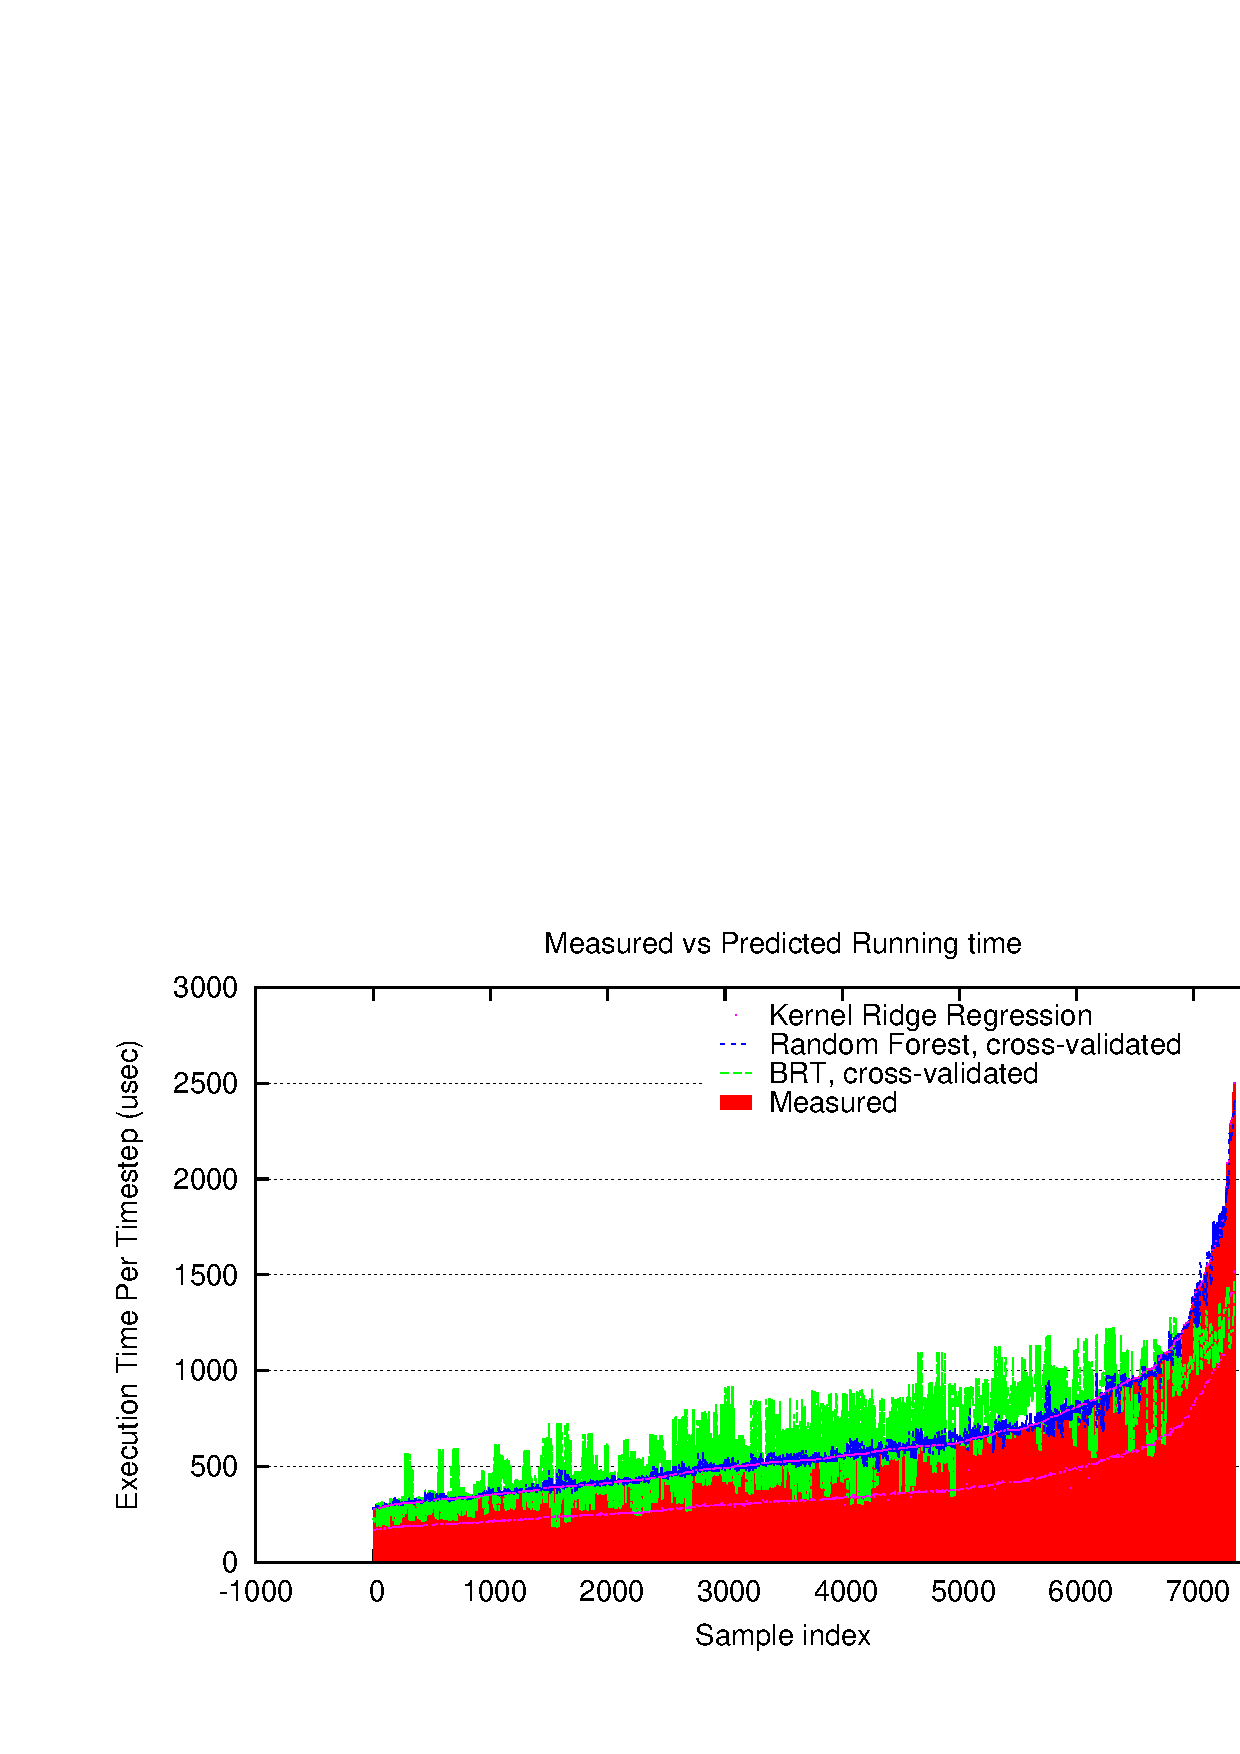
\includegraphics[width=\textwidth]{images/simple-cmp}
    \caption{Simple Stencil}
    \label{fig:simple-compare}
  \end{subfigure}
	%
  ~ %add desired spacing between images, e. g. ~, \quad, \qquad etc.
    %(or a blank line to force the subfigure onto a new line)
  \begin{subfigure}[b]{0.8\textwidth}
    \centering
    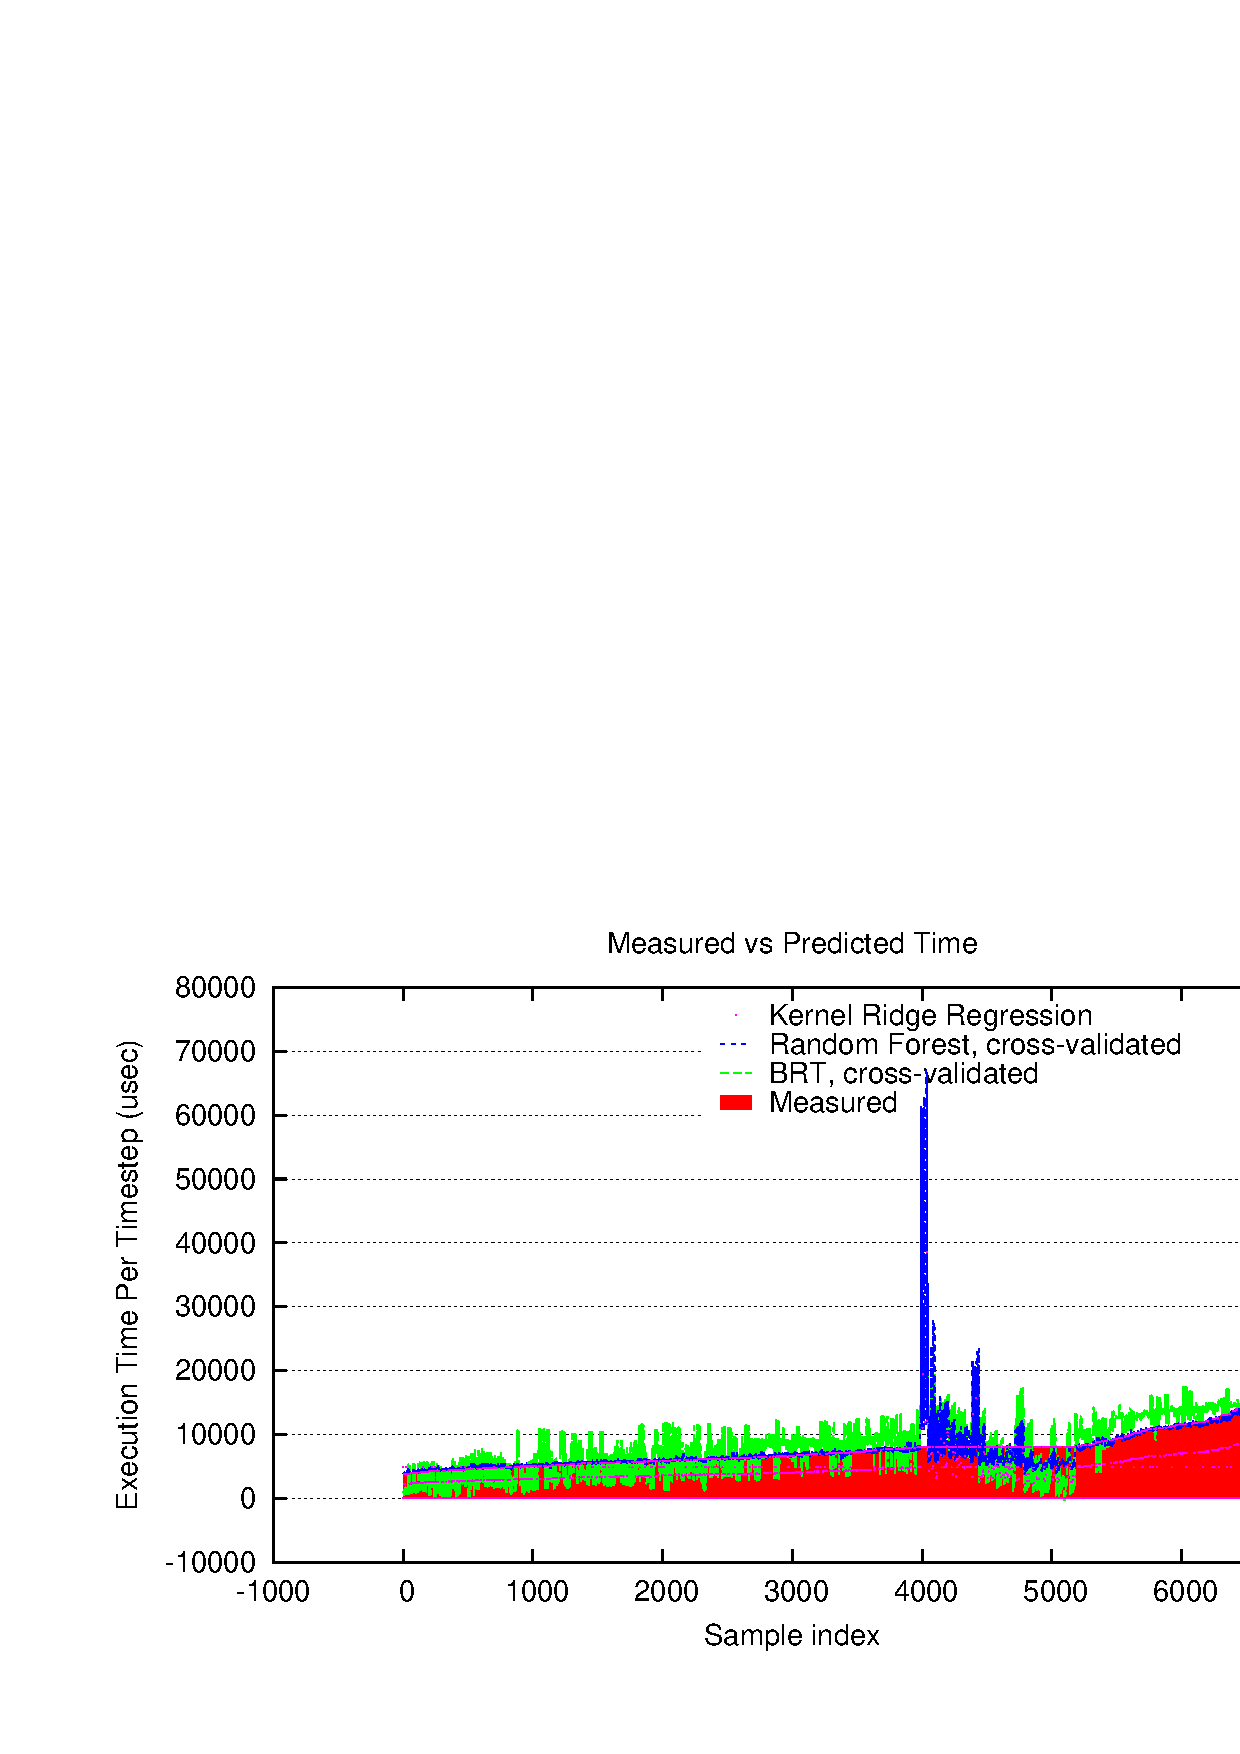
\includegraphics[width=\textwidth]{images/hypterm-cmp}
    \caption{Hypterm Kernel}
    \label{fig:hypterm-compare}
  \end{subfigure}
  \caption{Comparision of predicted results of Gradient Boosted Regression Tree, Kernel Ridge Regression, and Random Forest.}
\label{fig:compare}
\end{figure*}

Now let us proceed to see how well they are in action. I use Hill-Climbing algorithm for 75 iterations to search for best configurations for Gradient Boosted Regression Tree, Random Forest, and Kernel Ridge Regression. And use the same genetic algorithm with KCCA as Ganapathi et al.\ Table \ref{table:simple} and Table \ref{table:hypterm} shows the best running time of all the machine learning algorithms in Simple Stencil and Hypterm kernel, respectively. The columns are arranged from worst to best performance. The average running time comparison plot is also shown in Figure \ref{fig:compare_all}. KCCA is in a league of its own, with the average case 0.1\% away from the best configurations in simple stencil and 0.3\% in Hypterm kernel. Random Forest is the second best despite its spike. Gradient Boosted Regression Tree does hold itself. Kernel Ridge Regression tree lagging behind so badly is not very surprising considering the model is quite simple. However, this might also be me choosing wrong kernel too.

\begin{table}[ht]
\caption{Simple Stencil Kernel Tuning Results (Time in Microseconds)}
\center
\begin{tabular}{r c c c c}
\hline
 & KRR	& GBRT	& Random Forest	& KCCA \\
\hline\hline
Average	& 684.4274	& 303.2128	& 302.9823	& 275.5940 \\
Minimum	& 277.1379	& 275.3037	& 275.3037	& 275.3037 \\
Maximum	& 1958.7149	& 324.6784	& 324.7757	& 276.9702 \\
Standard Deviation	& 296.2554	& 15.1116	& 15.1782	& 0.5464 \\
\% error of Average from Optimal	& 148.6082	& 10.1376	& 10.0538	& 0.1054 \\
\cline{2-5}
Training Time & 0.5208 & 0.7000 & 0.1380 & 0.2664 \\
Prediction Time & 457.5783 & 461.0703 & 421.3316 & sth \\
Average \#Tests & 75 & 75 & 75 & 16.67 \\
\hline
\end{tabular}
\label{table:simple}
\end{table}

\begin{table}[ht]
\caption{Hypterm Kernel Tuning Results (Time in Microseconds)}
\center
\begin{tabular}{r c c c c}
\hline
 & KRR	& GBRT	& Random Forest	& KCCA \\
\hline\hline
Average	& 6927.8448	& 4205.2489	& 4088.5444	& 3723.5620 \\
Minimum	& 3770.1504	& 3711.3638	& 3711.3638	& 3715.6557 \\
Maximum	& 73002.4738	& 8037.9917	& 8037.9917	& 3764.0666 \\
Standard Deviation	& 4520.2231	& 909.3400	& 635.4020	& 17.1137 \\
\% error of Average from Optimal	& 86.6657	& 13.3074	& 10.1629	& 0.3287 \\
\cline{2-5}
Training Time & 0.4751 & 0.7095 & 0.1331 & 0.2774 \\
Prediction Time & 545.5813 & 453.0949 & 512.3045 & 157.7211 \\
Average \#Tests & 75 & 75 & 75 & 22.67 \\
\hline
\end{tabular}
\label{table:simple}
\end{table}

\begin{figure*}[h]
\centering
\includegraphics[width=0.8\textwidth]{./images/compare_all.pdf}
\caption{Comparison of all machine learning methods on both simple stencil and Hypterm kernels}
\label{fig:compare_all}
\end{figure*}

Other factor to be concerned is time, however, in this project the largest number of training set is 1000, at which even KCCA takes about the same time as other algorithms. How we would trade-off the tuning ability with time would be an interesting topic to be explored later, as performance of tree algorithms usually get better with increasing number of samples. But as of now if we have around thousands of samples, I would definitely choose KCCA, then Random Forest, and then Boosted Regression Tree.


\pagebreak
\section{Conclusion}

This paper has presented three direct interaction N-Body algorithms as well as proofs of their communication optimality. All algorithms provide the opportunity to minimize latency and bandwidth by utilizing extra memory. We also showed that they yield modest speedups on communication-bound problem instances. Our algorithms provide significantly better strong scaling, and consequently they can be scaled to larger machines without incurring substantial communication overhead.


\bibliographystyle{abbrv}
\bibliography{references}

\end{document}
